\chapter{NuSTORM beam neutrino interaction studies}
\label{c:neutrinoNuSTORM}

The Baby MIND is build to reconstruct muon tracks passing through the detector, this makes it ideal to be used for muon neutrino reconstruction with an appropriate target. As discussed in subsection~\ref{subsection:Neutrino interactions} there are only a few interactions which produce a free muon which can then be reconstructed with the Baby MIND. These are the muon neutrino charge current interactions, quasi-elastic charge current interactions, deep inelastic scattering and resonant interactions each at various energy ranges as can be seen in \FigRef{fig:neutrinoInteractionsFig} and in \FigRef{fig:antineutrinoInteractionsFig} 

\begin{figure}[h!]
\centering
\includegraphics[width=0.9\textwidth]{figures/figs_zeller-total-numode.png}
\caption{Neutrino cross sections, showing the quasi-elastic, deep inelastic and single pion cross sections in the GeV range. Taken from~\cite{82McFarland} modified from original made by G.P.~Zeller~\cite{106Zeller} containing data points from various experiments.}
\label{fig:neutrinoInteractionsFig}
\end{figure}

\begin{figure}[h!]
\centering
\includegraphics[width=0.9\textwidth]{figures/antineutrinototal.jpeg}
\caption{Antineutrino cross sections, showing the quasi-elastic, deep inelastic and single pion cross sections in the GeV range~\cite{109Formaggio}.}
\label{fig:antineutrinoInteractionsFig}
\end{figure}

The signature for each of these interactions are quite different as a charge-current quasi-elastic interaction will produce a clean proton and muon track, compared to a shower like pion track or the less clear DIS signature. Baby MIND is designed to operate at a lower energy spectrum, below 5 GeV, meaning that the contribution will be mostly from CCQE and pion interactions. Results from various simulations with the T2K near detector beam spectrum and data recorded from the commissioning will be showed.

%Lab report again, trying to estimate cross-section of interactions. Why? Need it to improve oscillation measurements. Using simulations of muon neutrinos from simulation. What is done, what cuts? How Do we calculate cross-sections? Angular acceptance, look at what Marc has done, do similar things and further the calculations.Discuss what to expect, what kind of interactions could happen in the TASD/WAGASCI? What could be seen? What information? Baby MIND can also have interactions, which ones would be visible? Can reconstruct muons in Baby MIND, electrons and pions visible and potentially reconstructable, but not now. Charge id, momentum. Identifying muons comming of the neutrino interaction with a specific beam and interaction area. Describe the fiducial volume like in my talk for NuFACT.

\section{Muon charge current quasi-elastic}

CCQE interactions produce a clear muon track for both neutrinos and anti-neutrinos, however the interaction only produces a proton track for neutrino interactions as seen below:
\begin{align}
\nu_\mu + n &\rightarrow \mu^- + p\\
 \bar{\nu_\mu} + p &\rightarrow \mu^+ + n
\end{align}

For the neutrino interactions, this becomes a very clear signature in a fully active target where both a muon and proton track can be identified. For anti-neutrinos this is not possible since neutron tracks are usually not detectable for most detector types. However the main goal is to identify muon tracks from pion tracks which is simply identifying a shower from a track. There have been a lot of interesting articles relating to how to identify neutrino events in Argon detectors using machine learning~\cite{83Radovic2018}~\cite{84Adams}. In a non active target it becomes very difficult to identify neutrino interactions as pions may decay to muons and become indistinguishable from directly produced muons.

%Direct simulations with CCQE and different geometries. Use data from specifically Baby MIND in B2 beam line. Explain the beam line etc etc.

%CCQE from muon neutrino produces a muon. Clear production and easy to identify in TASD, not possible in MIND due to the design. 

%Acceptance study, detector layout. Beam settings? Add charge reconstruction, momentum reconstruction. Particle ID? also need interaction ID from TMVA.

%Different size gap, different detector layout both early/testbeam and new at Japan. Cross-section studies. Look at what Marc has done!  Discuss with paul what and how to do cross-section measurements.

\pagebreak
\subsection{Interactions in TASD + Baby MIND}

As described in subsection~\ref{subsec:NuSTORM}, a first stage towards a neutrino factory would contain a storage ring for neutrino and anti-neutrino production from muon decay. From a muon decay both muon and anti-electron neutrinos will be produced at $\approx 100\%$. In this study the TASD and Baby MIND has been used as a near detector to measure the interaction type and reconstruction of muon tracks. The main study is to see if it is possible to identify muon neutrino charge current quasi elastic (CCQE) interactions in a background of neutral current interactions and anti-electron charge current interactions. This is done using a TMVA trained algorithm with simulated samples. As part of this study the fitted efficiency and charge identification efficiency of muon and anti-muon tracks produced by simulated muon and anti-neutrinos in Baby MIND is shown.

The NuSTORM neutrino energy spectrum has been simulated as can be seen in \FigRef{fig:NuSTORMeSpectrum} for both muon and anti-electron neutrinos. The main job for any detector will be to identify if the neutrino event is produced from either a muon interaction or an electron interaction as well as dealing with the small background ($<1\%$) of anti-muon produced electron and anti-muon neutrinos.

\begin{figure}[h!]
\centering
\includegraphics[width=0.9\textwidth]{figures/eSpectrum.pdf}
\caption{Energy spectrum of muon and anti-electron neutrinos produced at NuSTORM and recorded at 50 m from the storage ring.}
\label{fig:NuSTORMeSpectrum}
\end{figure}

During the construction of Baby MIND, it was proposed to potentially fully instrument the whole TASD, used during the first beam test, and use it as a fully active target to be combined with Baby MIND, illustrated in~\FigRef{fig:TASDandMIND}. This would become a setup for a NuSTORM detector.

\begin{figure}[h!]
\centering
\includegraphics[width=0.9\textwidth]{figures/MINDAida.jpeg}
\caption{An illustrative sketch of the detector setup with the TASD detector in front of Baby MIND.}
\label{fig:TASDandMIND}
\end{figure}

Figures of merit for the muon neutrino study are presented below.In \FigRef{fig:NuSTORMTASDfitted} the fitted efficiency is presented, \FigRef{fig:NuSTORMTASDfittedcharge} shows the charge efficiency and finally \FigRef{fig:NuSTORMTASDCombined} shows these two multiplied. Each of the plots show different metrics to evaluate the SAURON framework and the detector performance. The fitted efficiency is defined as the ratio of reconstructible tracks divided by all the simulated tracks. The charge efficiency is defined as how many of the reconstructible tracks are reconstructed with the correct charge. Multiplying these two results in the ratio of correctly charge reconstructed tracks divided by all simulated tracks.

\begin{figure}[h!]
\centering
%\includegraphics[width=.9\textwidth]{figures/NeutrinoChap/data260618/T2K/FittedT2KNeutrinoBeamMIND.pdf}
\includegraphics[width=.9\textwidth]{figures/NeutrinoChap/Neutrino/NuStormRecEff.pdf}
\caption{The efficiency plot of how well the algorithm can reconstruct neutrino tracks vs muon momenta for simulated tracks interacting in the TASD.}
\label{fig:NuSTORMTASDfitted}
\end{figure}

\begin{figure}[h!]
\centering
\includegraphics[width=.9\textwidth]{figures/NeutrinoChap/Neutrino/NuStormChargeEff.pdf}
%\includegraphics[width=.9\textwidth]{figures/NeutrinoChap/data260618/T2K/ChargeIDT2KNeutrinoBeamMIND.pdf}
\caption{The efficiency plot of how well the algorithm can reconstruct muon charge vs muon momenta for tracks fitted in the algorithm.}
\label{fig:NuSTORMTASDfittedcharge}
\end{figure}

\begin{figure}[h!]
\centering
\includegraphics[width=.9\textwidth]{figures/NeutrinoChap/CombinedNuStormChargeFittedEff.pdf}
%\includegraphics[width=.9\textwidth]{figures/NeutrinoChap/data260618/T2K/ChargeIDT2KNeutrinoBeamMIND.pdf}
\caption{The efficiency plot of how well the algorithm can reconstruct muon charge vs muon momenta for simulated tracks. Combination of the previous two figures.}
\label{fig:NuSTORMTASDCombined}
\end{figure}

Similarly to the simulated muon beam, and data the charge reconstruction efficiency is very good for the reconstructible tracks. The difference comes from the fact that the neutrinos are produced at angles instead of straight on the center of the detector (with some beam size). Muons from neutrinos are produced at all angles depending on the kinematics of the neutrino interaction and neutrino energy. 

For the TMVA algorithm, similar variables to the muon, pion study for the test beam as to simplify the implementation.

The main variables used in the model are the following:
\begin{itemize}
\item Maximum distance between hits in an event / Naive track length
\item Angle of the track compared to a straight line into the detector
\item Number of total hits in the event
\item Number of planes hit
\item Average number of hits per plane
%\item Number of total hits,
%\item Number of used planes for fit
%\item Number of hits used for fit/ number of used planes
%\item Average number of hits per plane
%\item Maximum distance between hits in an event / Naive track length
\end{itemize}

The distributions of these variables for signal and background can be seen in \FigRef{fig:TMVANeuinput}.


\begin{figure}[h!]
\centering

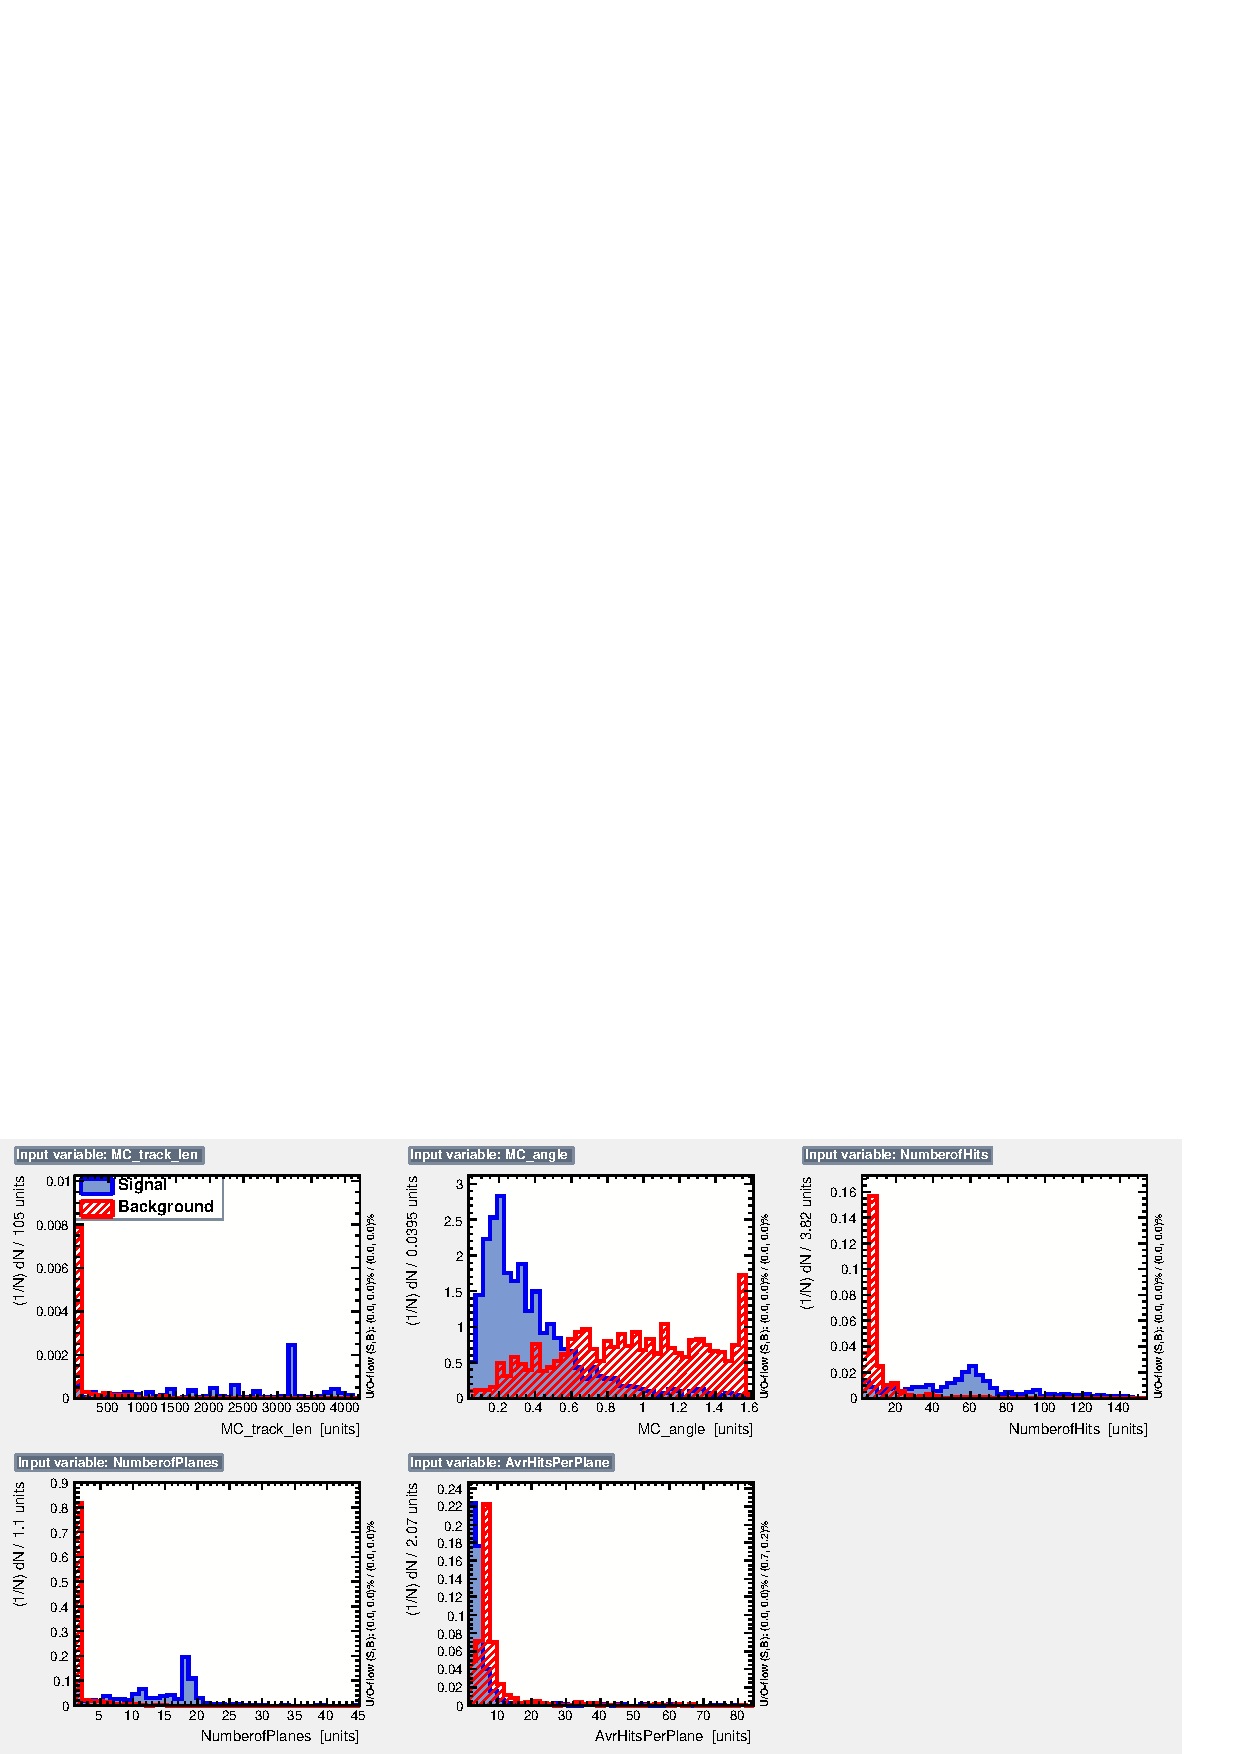
\includegraphics[width=\textwidth]{figures/neutrinoTMVA/variables_id_c1.png}
\caption{Input variables for both signal and background using simulated data}
\label{fig:TMVANeuinput}
\end{figure}

Based on these simulated signal and background samples, TMVA will provided a Signal efficiency curve based on the various build in models, seen in \FigRef{fig:TMVANeuroc}. In this plot is is clear that several models outperform others, however the multilayer perception with a Bayesian Neural Network (MLPBNN) was choose as the best performing model. The MLPBNN response can be seen in \FigRef{fig:TMVANeuresponce} and shows a clear distinction between signal and background samples. It is quite clear that any cut between these two distinct peaks will produce the desired outcome, this is plotted in \FigRef{fig:TMVANeucuts} and shows the ideal value if the number of signal and background events are equal.


%Currently found that the best method, however many perform similarly, is MLPBNN, Multilayer perceptron (neutral network) with BFGS training method, similar to gradient decent or quasi-Newton method, and bayesian regulator.


\begin{figure}[h!]
\centering

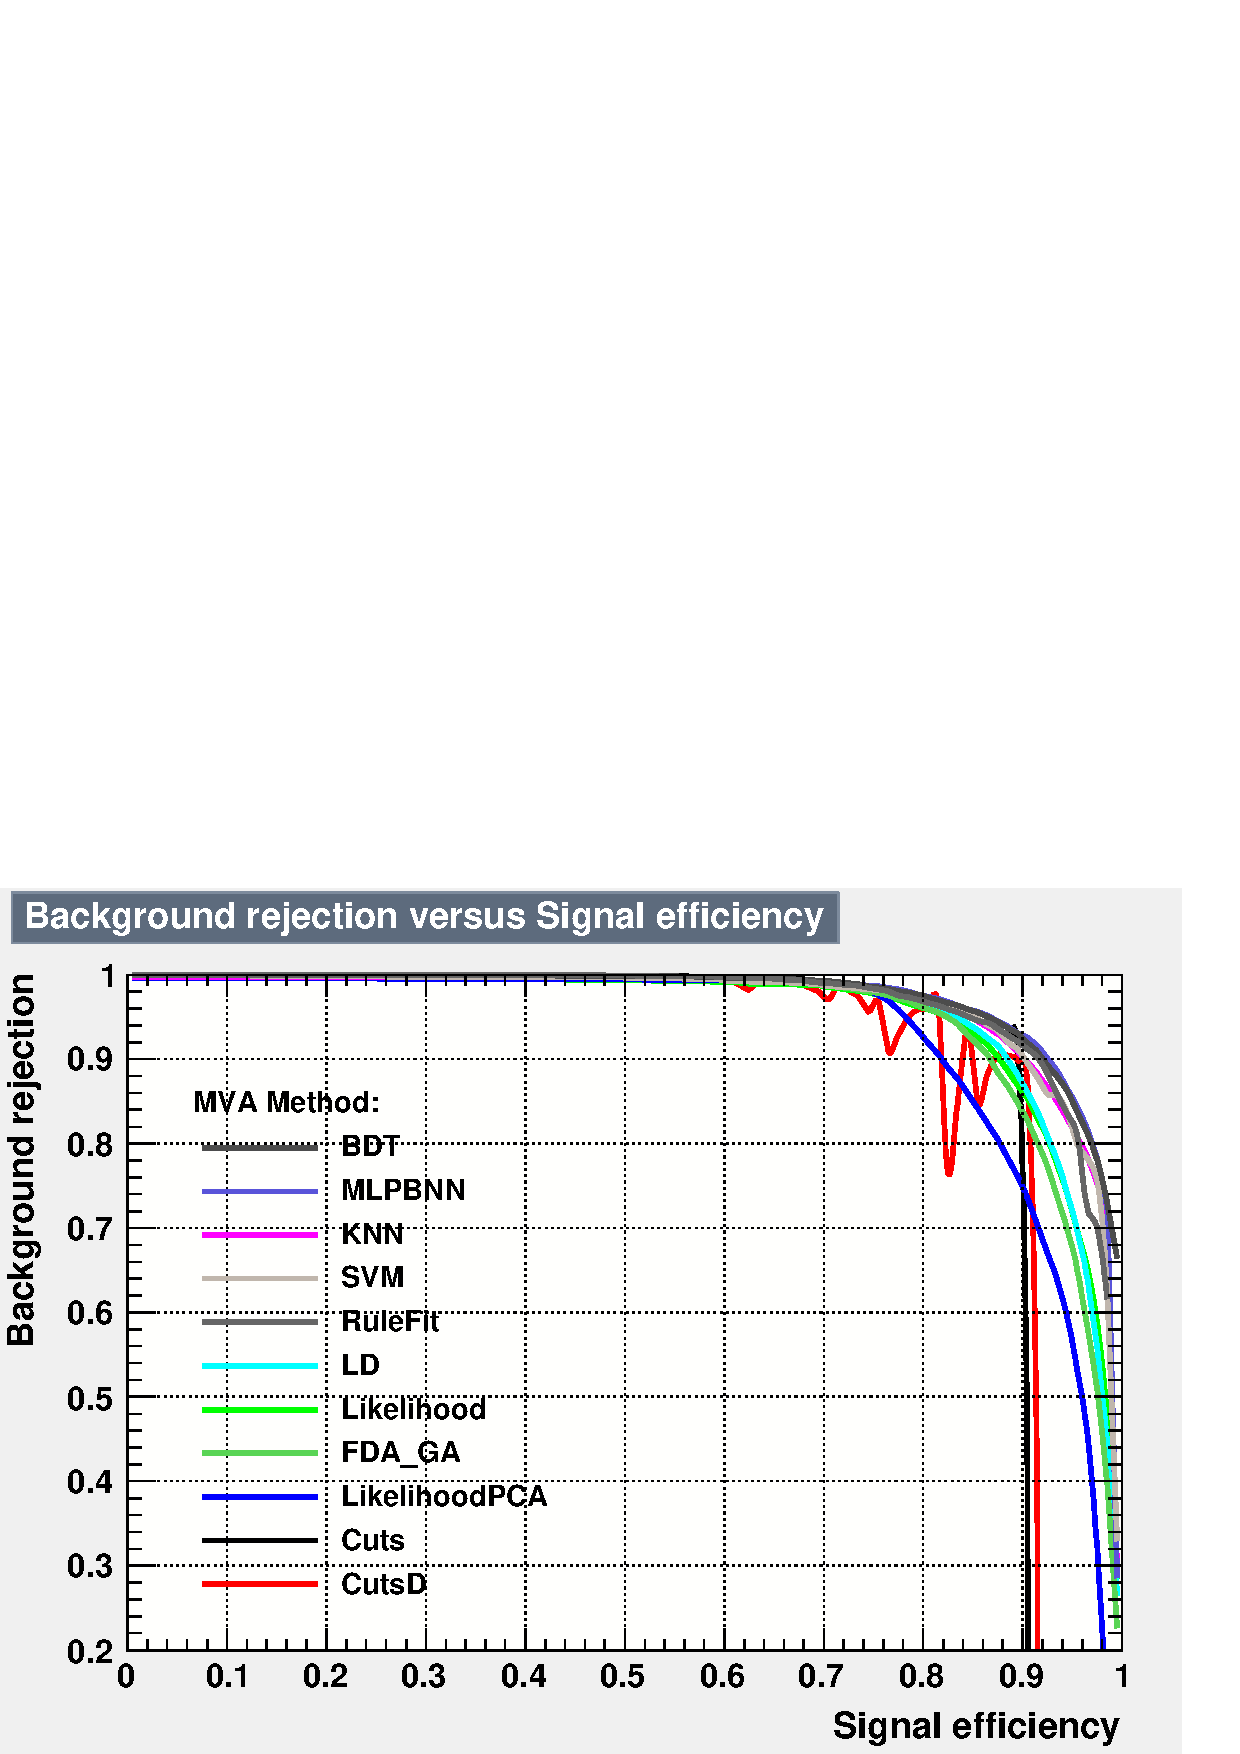
\includegraphics[width=\textwidth]{figures/neutrinoTMVA/rejBvsS.png}
\caption{ROC curve for various machine learning algorithms.}
\label{fig:TMVANeuroc}
\end{figure}

\begin{figure}[h!]
\centering
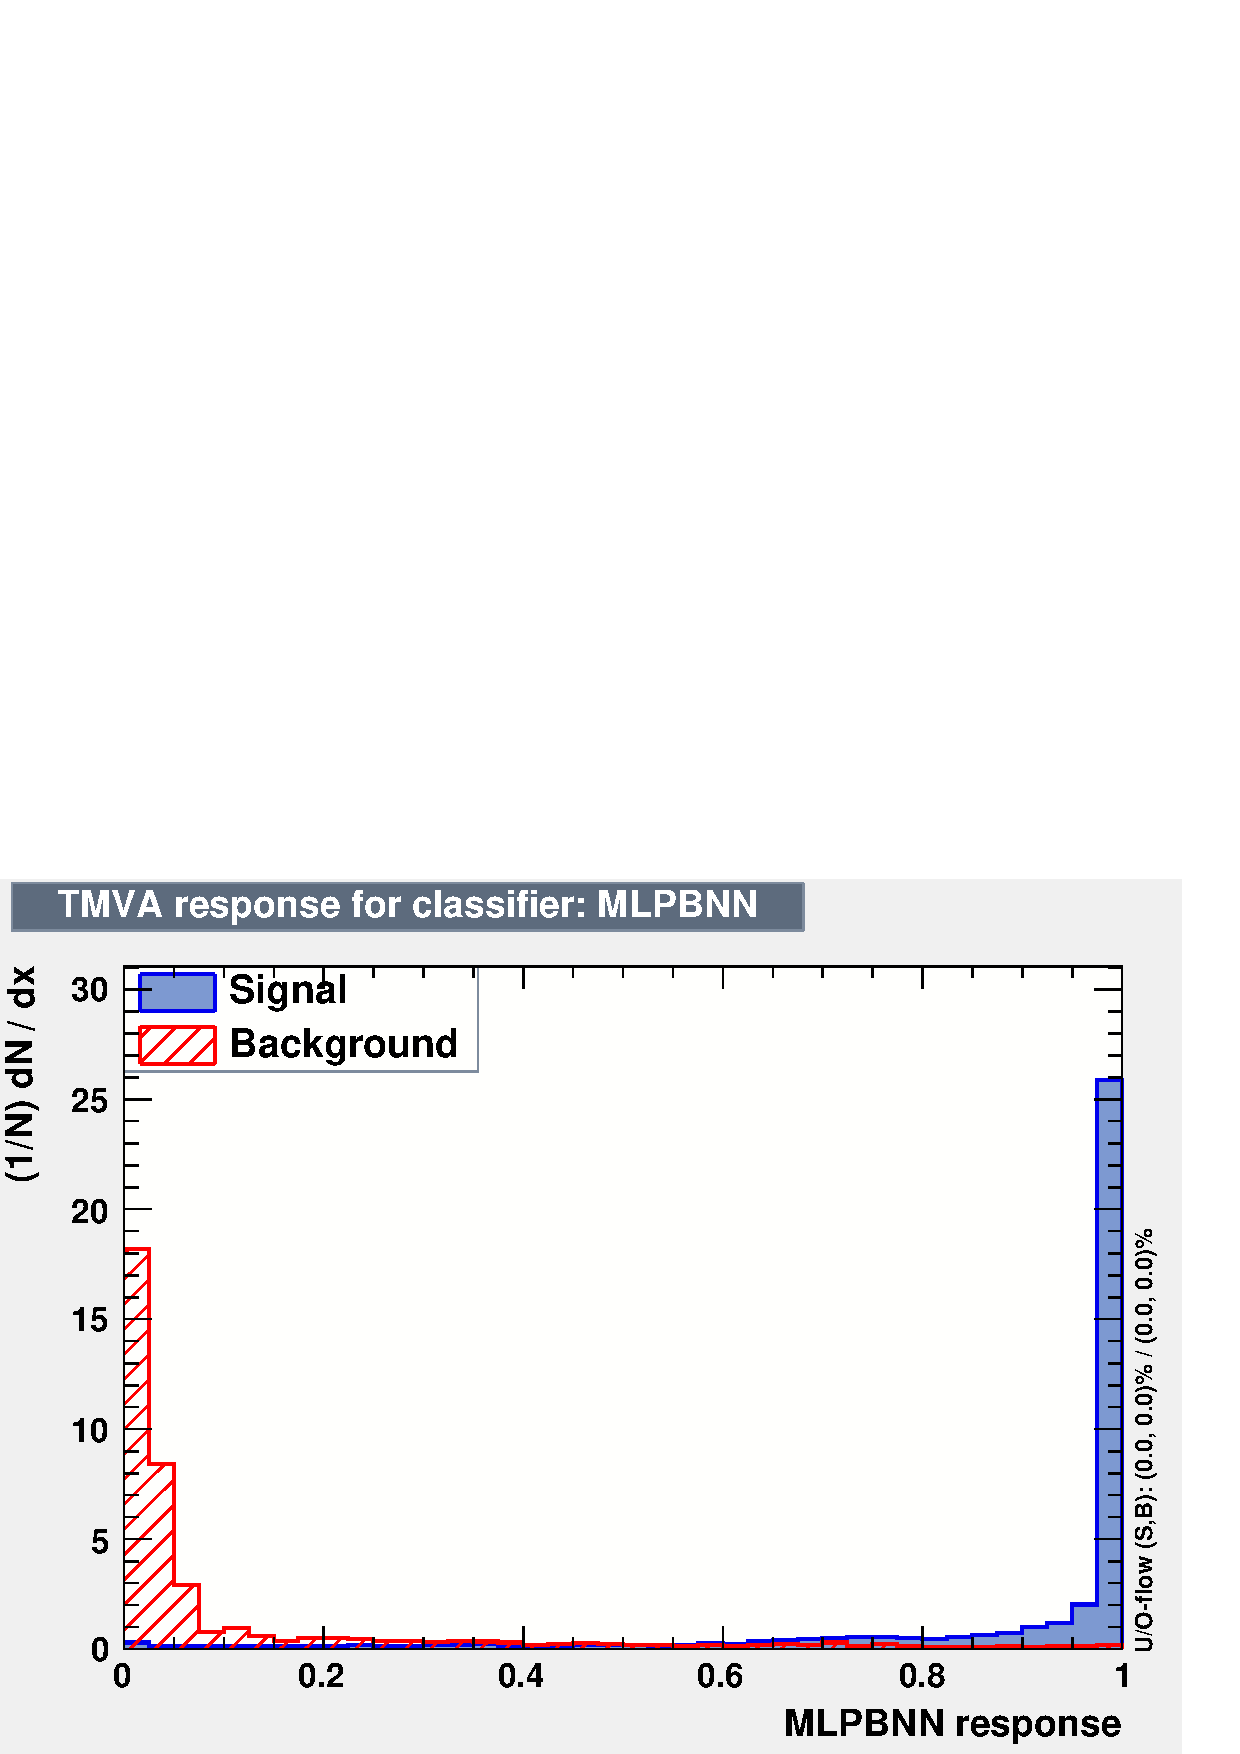
\includegraphics[width=.49\textwidth]{figures/neutrinoTMVA/mva_MLPBNN.png}
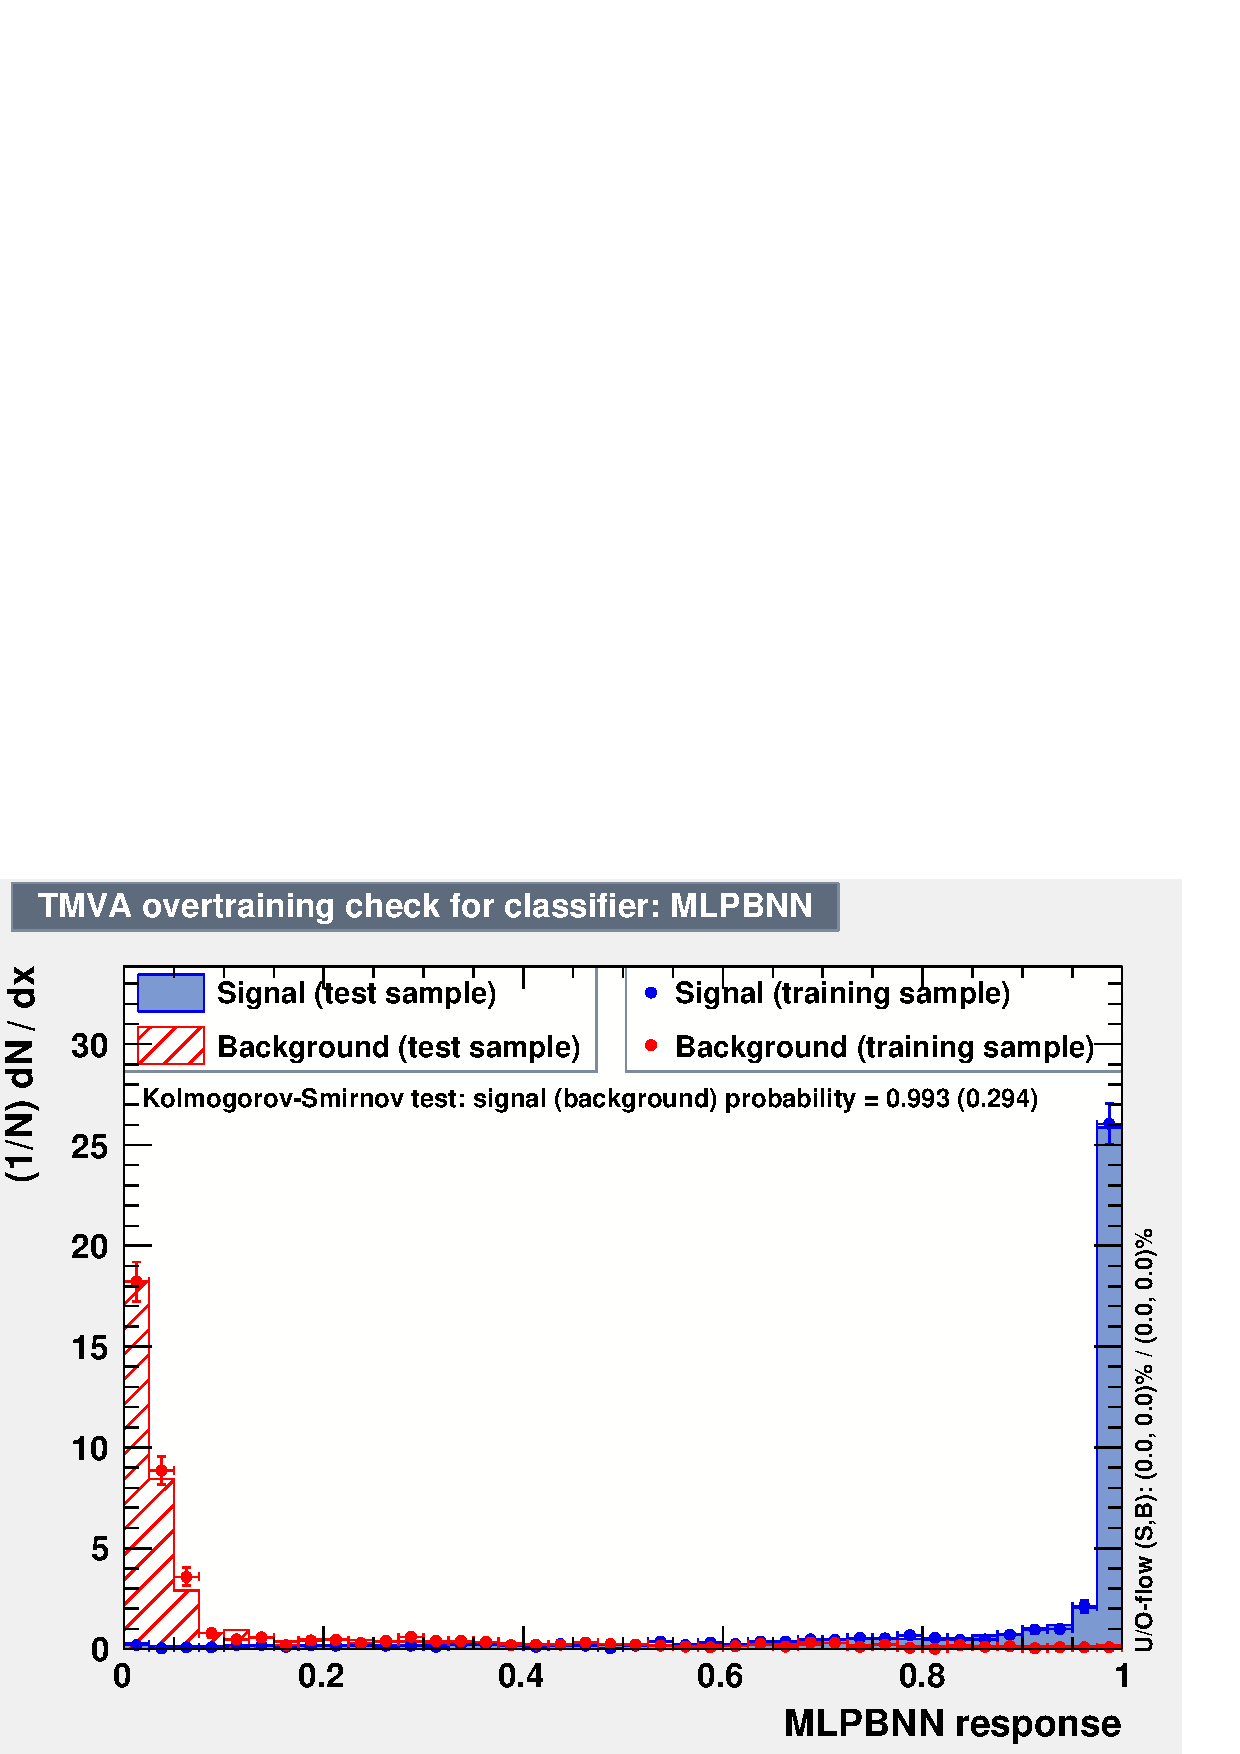
\includegraphics[width=.49\textwidth]{figures/neutrinoTMVA/overtrain_MLPBNN.png}
\caption{Response with and without over-training check}
\label{fig:TMVANeuresponce}
\end{figure}

With this trained algorithm the best possible cut value provides 91.3 \% of the signal to pass through in a pure sample of signal events and only 7.5 \% of background events in a pure background event sample. As with the previous study this is done independent of neutrino energy values. This could be improved by looking at specific energy values and by looking at more variables to used such as perhaps energy deposited into the scintillating bars in the detector, however this would require a further study to determine potentially better variables.

Applying the TMVA algorithm to a mixed sample of electron neutrinos and muon neutrinos produces the neutrino energy spectrum seen in \FigRef{fig:TMVAEspectrumAfter} with the initial spectrum seen in \FigRef{fig:TMVAEspectrumBefore}.


\begin{figure}[h!]
\centering
\includegraphics[width=\textwidth]{figures/NeutrinoChap/mvaeffs_MLPBNN10001300.png}
%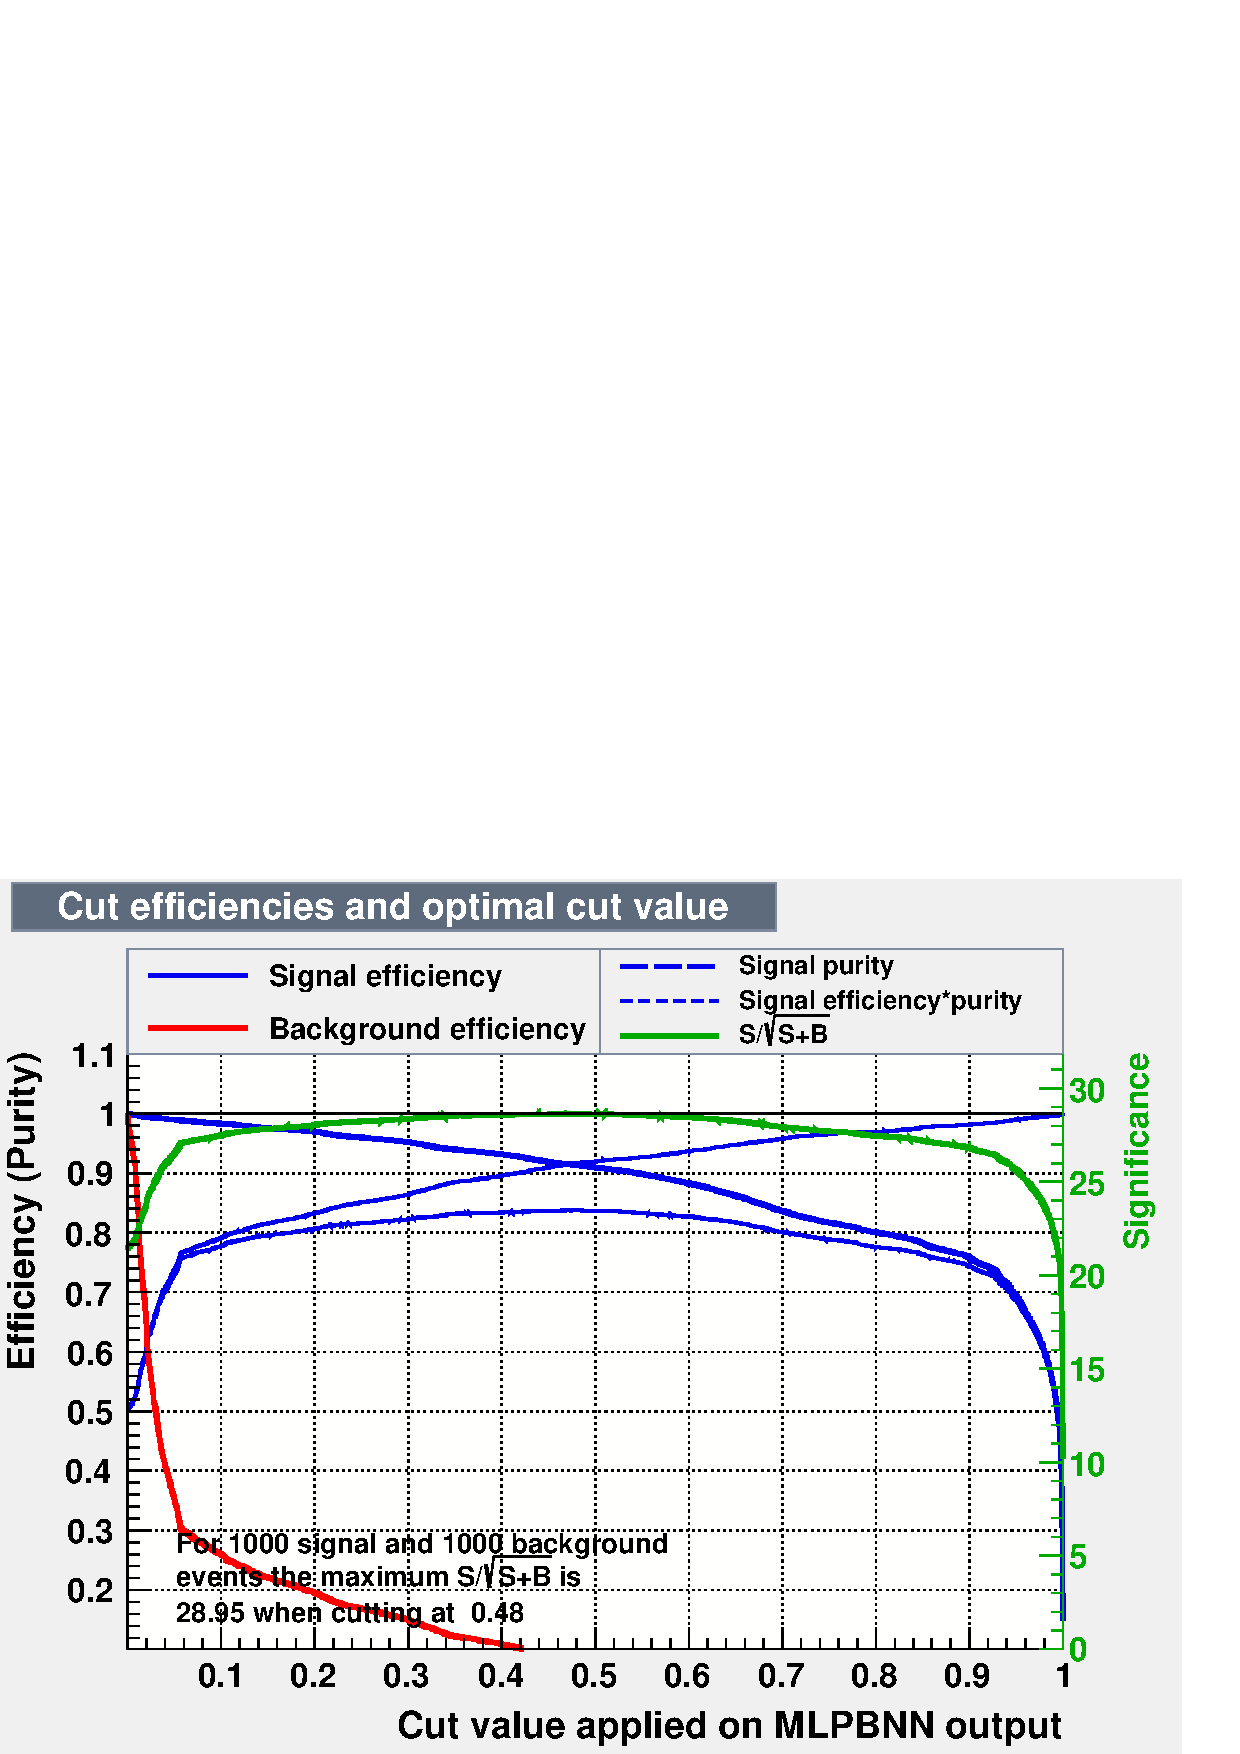
\includegraphics[width=\textwidth]{figures/neutrinoTMVA/mvaeffs_MLPBNN.png}
\caption{Cut efficiency plots expecting the combined background of $\bar{\nu_{e_{CC}}}$ to be at the same number as the signal ($\nu_{\mu_{CC}}$) and $\nu_{\mu_{NC}}$ to be approximately $\frac{1}{3}$ of the number of signal events. }
\label{fig:TMVANeucuts}
\end{figure}

\begin{figure}[h!]
\centering
\includegraphics[width=.9\textwidth]{figures/NeutrinoChap/SpectrumBeforeTMVA.pdf}
%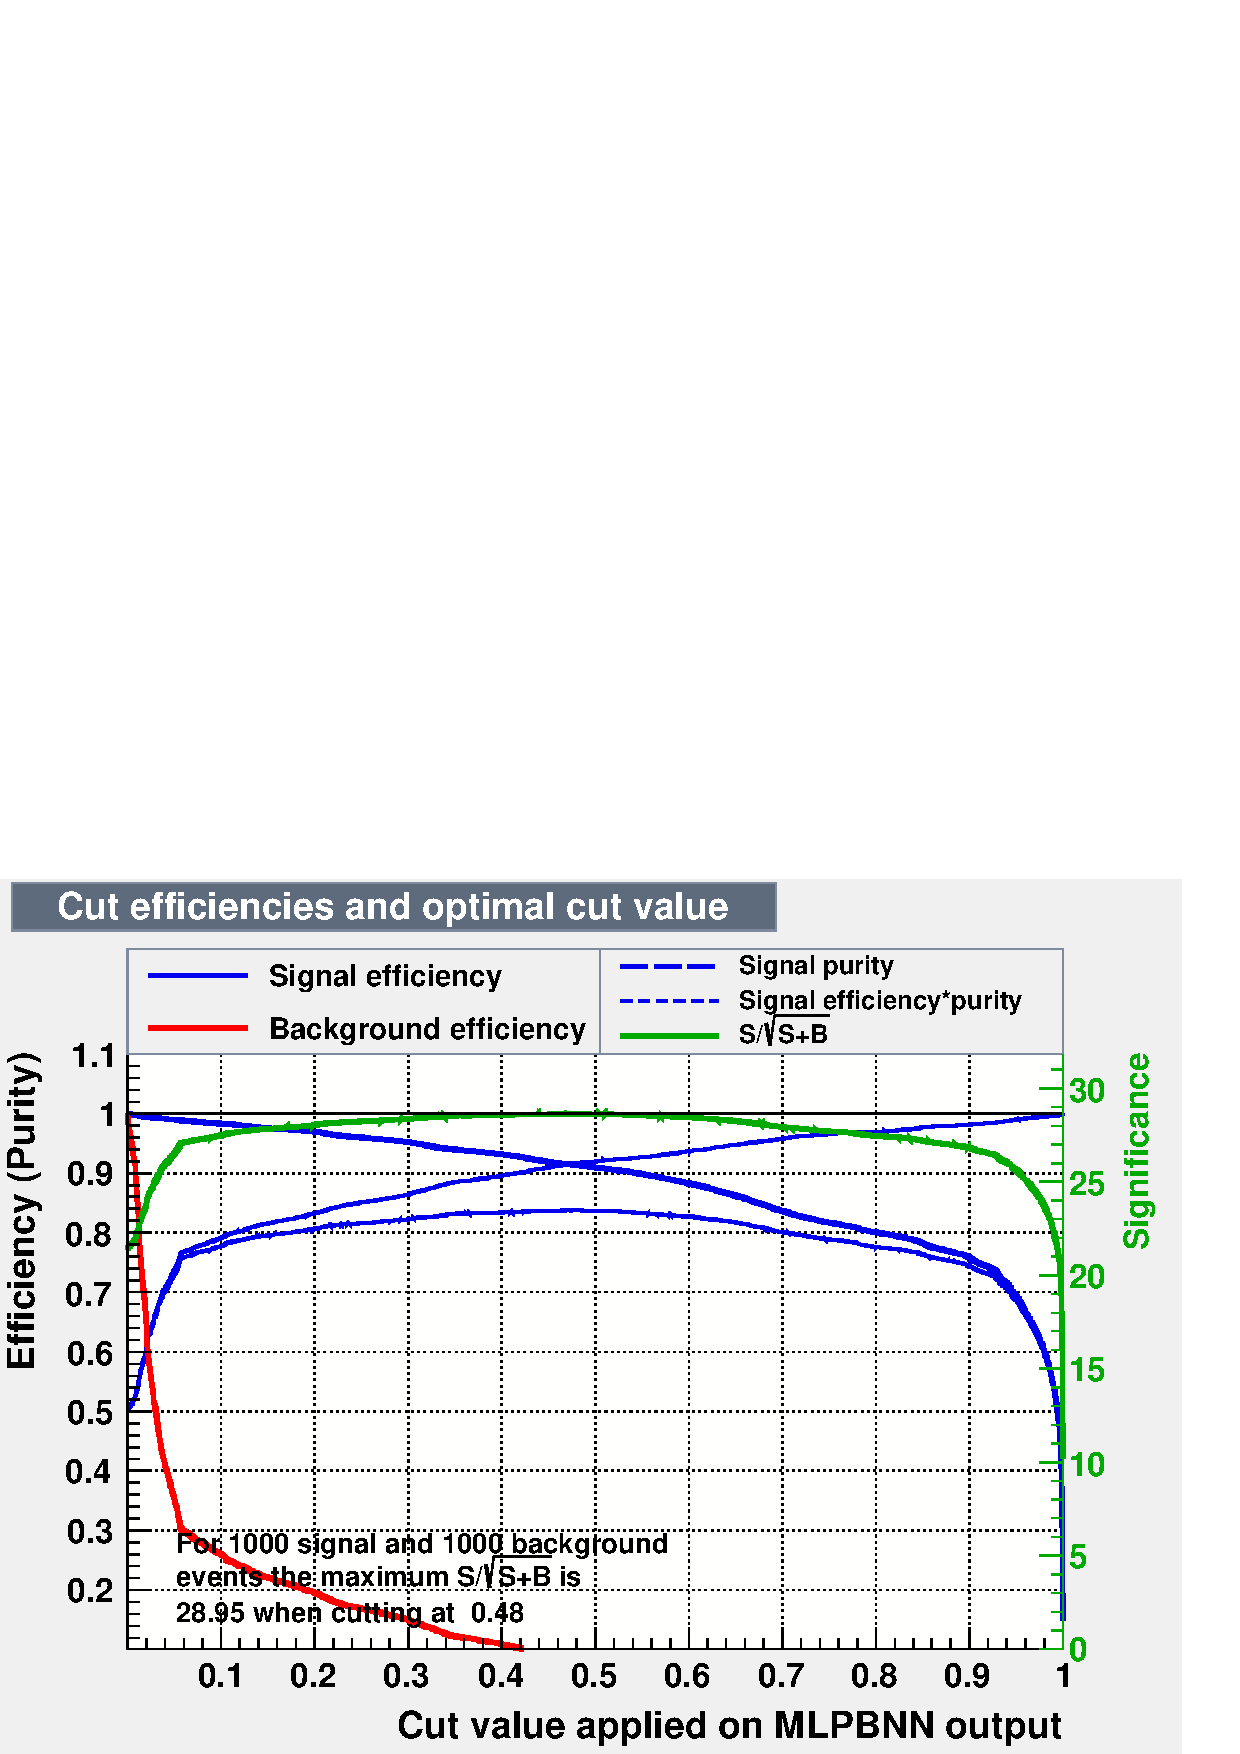
\includegraphics[width=\textwidth]{figures/neutrinoTMVA/mvaeffs_MLPBNN.png}
\caption{Neutrino energy spectrum of $\bar{\nu_{e_{CC}}}$ , $\nu_{\mu_{CC}}$ and $\nu_{\mu_{NC}}$ produced from $10^{20}$ POT, before passing through the TMVA algorithm.}
\label{fig:TMVAEspectrumBefore}
\end{figure}


\begin{figure}[h!]
\centering
\includegraphics[width=.9\textwidth]{figures/NeutrinoChap/SpectrumAfterTMVA.pdf}
%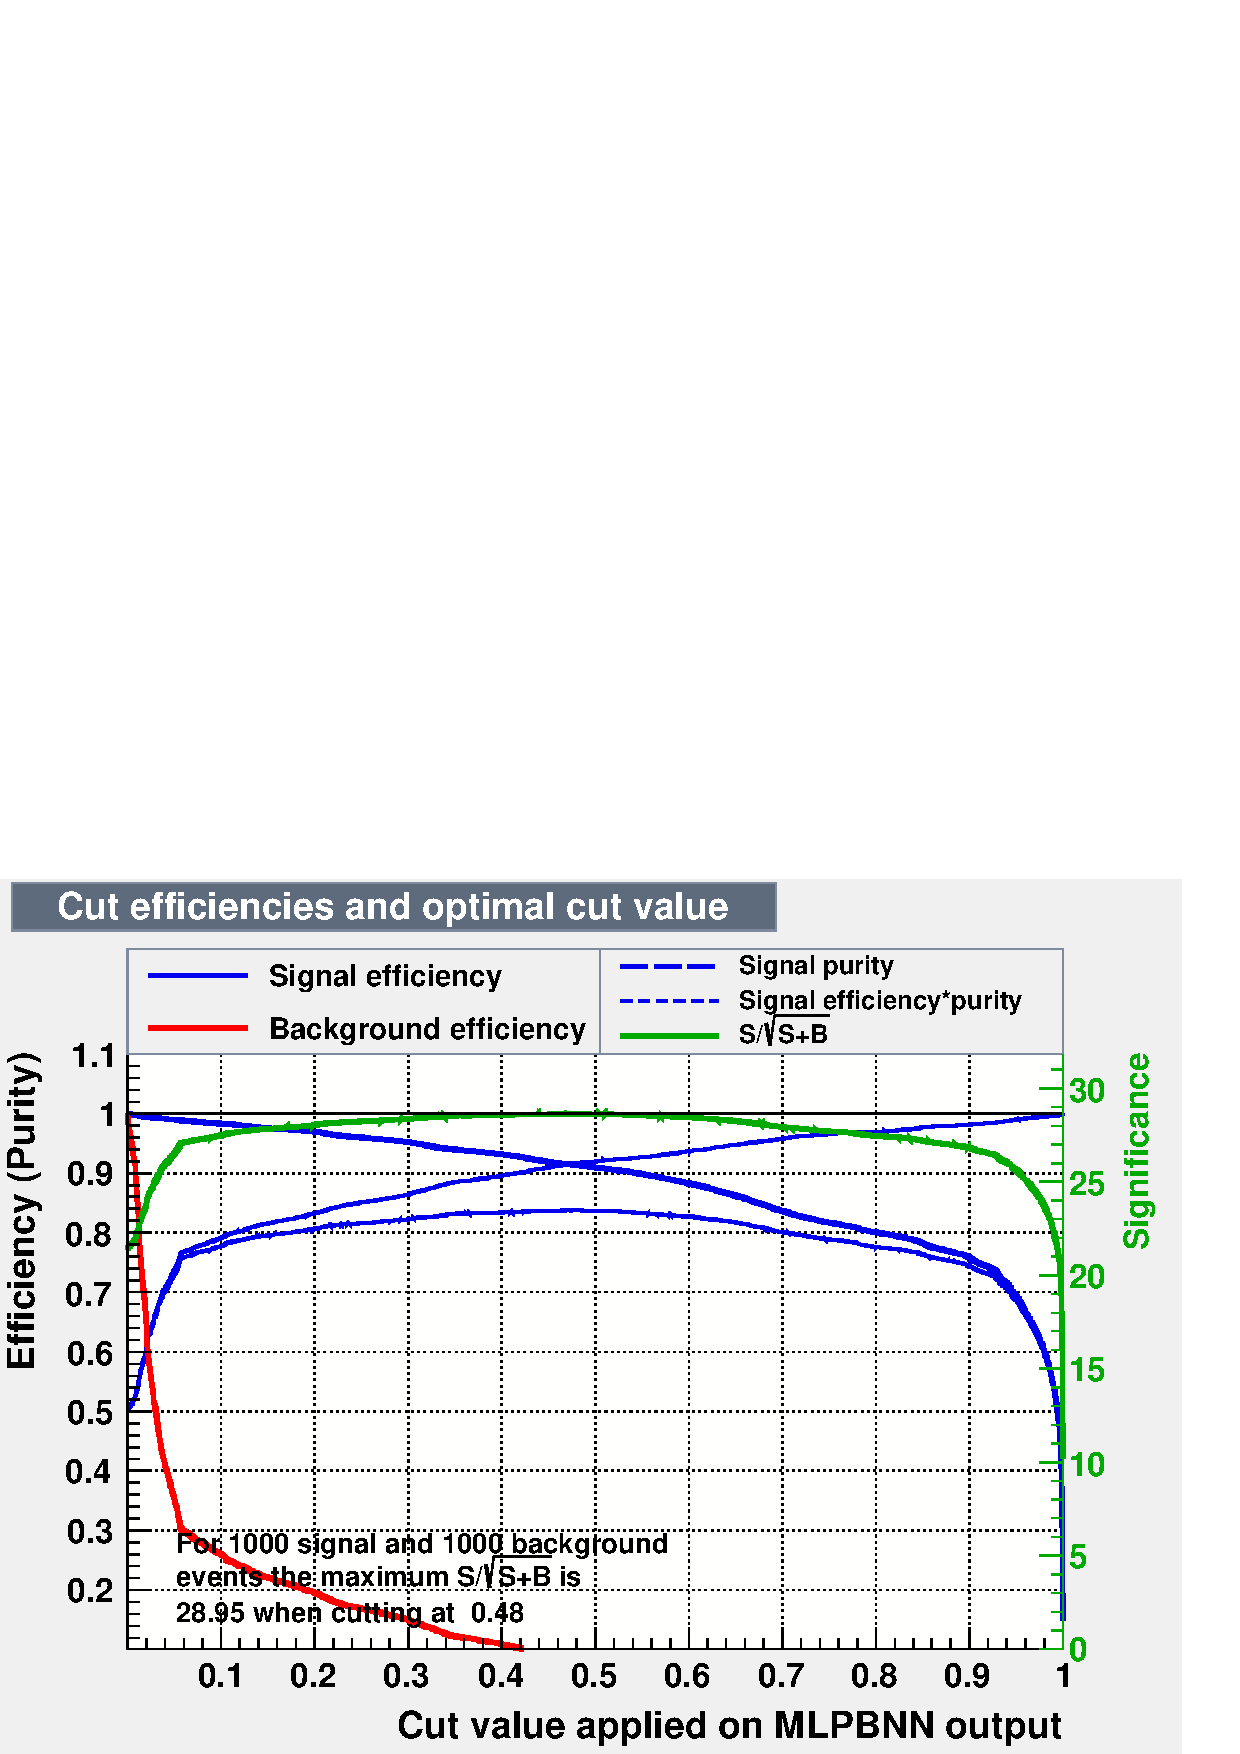
\includegraphics[width=\textwidth]{figures/neutrinoTMVA/mvaeffs_MLPBNN.png}
\caption{Neutrino energy spectrum of $\bar{\nu_{e_{CC}}}$, $\nu_{\mu_{CC}}$and $\nu_{\mu_{NC}}$ produced from $10^{20}$ POT, after passing through the TMVA algorithm.}
\label{fig:TMVAEspectrumAfter}
\end{figure}


%Describe the NuSTORM beam line again, expected energy of neutrinos.

%Interactions in the TASD, what would be the efficiency of identifying mu CCQE events in a background e CC and mu NC ? 

%New MC study using TMVA again, show plots and work. Show training and testing samples. Create mixed sample and show how well it can identify the parts. 

\pagebreak
\newpage

\section{Summary}
From the NuSTORM study is it clear that a TASD + Baby MIND configuration would be able to provide charge reconstruction of tracks down to 400 GeV/c with the possibility to identify and distinguish between the $\nu_{\mu_{CC}}$ signal in a background of $\bar{\nu_{e_{CC}}}$ and $\nu_{\mu_{NC}}$ with 91.3 \% efficiency.


%\subsection{Interactions in TASD + Baby MIND T2K (Remove?)}
\pagebreak
\newpage
\chapter{J-PARC beam neutrino interaction studies}
\label{c:neutrinoT2K}

%During the construction of Baby MIND, it was proposed to potentially fully instrument the whole TASD, used during the first beam test, and use it as a fully active target to be combined with Baby MIND, illustrated in~\FigRef{fig:TASDandMIND2}.

%\begin{figure}[h!]
%\centering
%\includegraphics[width=0.9\textwidth]{figures/MINDAida.jpeg}
%\caption{An illustrative sketch of the detector setup with the TASD detector in front of Baby MIND.}
%\label{fig:TASDandMIND2}
%\end{figure}

%\subsection{Interactions in TASD + Baby MIND}

%For all analysis the TASD is used as a CCQE identification and neutrino veto, expecting two tracks (neutrino) or atleast start of muon track. The dimensions are the same as mentioned under the test beam section, with a distance of 368mm between the two detectors. Neutrinos are simulated using the T2K near detector spectrum in reverse horn current mode (RHC), seen in~\FigRef{fig:T2KndSpectrum} in the SAURON framework. 

%Dont actually have the plots?

%Reshow the muon beam? Discussion about angle etc...

%Have simulations both for T2K and NuSTORM beamline, describe both.
%Full analysis in MIND, only TASD as veto.
 %Shown at NuSTORM talk, fix momentum slightly.
 
%\FloatBarrier
%\pagebreak
%\newpage
\section{Neutrino interactions in Iron in Baby MIND}

The T2K energy spectrum is produced on-axis, off axis etc. The ND280 experiment uses the beam at a 2.5 degree off-axis angle which provides a narrower energy spectrum with a shifted peak energy as can be seen in \FigRef{fig:T2KAxis}. The energy spectrum at 1.5 deg off-axis, is narrower and have a peak at a lower energy than the on-axis spectrum. Which can be seen in \FigRef{fig:T2KAxis2} The WAGASCI 1.5 off-axis energy spectrum is shifted slightly higher than the 2.5 off-axis energy spectrum used for the ND280 experiment.

%previous narrower and lower peak than on-axis and slightly higher energy than 2.0 and 2.5 deg. as seen in plots from NuFact talk. Beam comes with two modes, forward horn current (FHC) with neutrinos produced and reverse horn current with anti-neutrinos produced.

\begin{figure}[h!]
\centering
\includegraphics[width=0.9\textwidth]{figures/NeutrinoChap/ND280vsWAGASCIspectrum.jpeg}
\caption{Neutrino energy spectrum for WAGASCI (red, off-axis 1.5 degree), ND280 (black, off-axis 2.5 degree). Peak energy at 1.5 degrees, 800 MeV, vs 600 MeV at 2.5 degrees.}
\label{fig:T2KAxis}
\end{figure}

\begin{figure}[h!]
\centering
\includegraphics[width=0.9\textwidth]{figures/NeutrinoChap/offAxisFlux.jpeg}
\caption{Neutrino energy spectrum for WAGASCI extrapolated to 295km for various off-axis degree values.}
\label{fig:T2KAxis2}
\end{figure}

For the simulations the WAGASCI spectrum has been used, and the combined spectrum of muon neutrinos and anti-neutrinos for reverse horn current can be seen in \FigRef{fig:T2KndSpectrum}.


%In the framework several figures of merit are produced, the muon energy spectrum, reconstructed muon energy spectrum, reconstructability of tracks vs energy and charge reconstruction vs energy. All of these figures of merit are shown in~\FigRef{fig:T2KTASDfitted} and~\FigRef{fig:T2KTASDfittedcharge}. In \FigRef{fig:T2KTASDfittedcharge} the efficiency does not start at 0 as the few tracks which have been fitted can provide a charge, however comparing this with the fitted it is clear this is a minority of tracks seen in \FigRef{fig:T2KTASDCombined} and \FigRef{fig:T2KTASDCombinedZoom}.

\begin{figure}[h!]
\centering
\includegraphics[width=0.9\textwidth]{figures/WAGASCIflux.jpeg}
\caption{The energy spectrum for muon neutrinos and muon anti-neutrinos in the T2K near detector RHC beam.}
\label{fig:T2KndSpectrum}
\end{figure}

%Similarly to the simulated muon beam, and data the charge reconstruction efficiency is very good for the reconstructible tracks. The difference comes from the fact that the neutrinos are produced at angles instead of straight on the center of the detector (with some beam size). Muons from neutrinos are produced at all angles depending on the kinematics of the neutrino interaction and neutrino energy. 
%Simulations for a  T2K like beam, explain the details and event selection, (None for simulation but easy enough with data). Use the specific fiducial volume. Set up at J-PARC, all the details with that.
%Lead into expected momentum reconstruction? Potential for tracks to be miss constrocted given angle etc etc. Even with cuts on no hit in first plate and hits after iron possible for sand muons to pass through. Tracks leaving would affect reconstruction. Angle and leaving, other than that is should be ok. Few events in total... Number of events sent to Paul, seems resonable.

To compare simulations with data taken for the commissioning run interactions had to be simulated in the iron of the Baby MIND due to the fact that the WAGASCI data taking can as of yet not be joined with the Baby MIND data. The fiducial volume is chosen to be in the first iron module seen in \FigRef{fig:MINDneutrinoLayout} as a1-3 as well as selecting part of the iron plate, as seen with further details in \FigRef{fig:MINDFiducial}. 

\begin{figure}
\centering
\includegraphics[width=\textwidth]{figures/NeutrinoChap/NuFactTalk/Layout300118.jpeg}
\caption{The layout of the MIND for the commissioning neutrino run.}
\label{fig:MINDneutrinoLayout}
\end{figure}

\begin{figure}
\centering
\includegraphics[width=\textwidth]{figures/NeutrinoChap/NuFactTalk/eventRateCheck.jpeg}
\caption{Details of the fiducial volume for the neutrino events to compare simulations with data.}
\label{fig:MINDFiducial}
\end{figure}

Similarly to the simulated neutrino beam interacting in the TASD, the charge reconstruction efficiency is very good for the reconstructible tracks. The difference comes from the fact that the neutrinos are produced in the iron and that process adds more uncertainty for the neutrinos entering the Baby MIND. Comparing this to data will also add the possibility of geo-neutrino and muons entering the detector from the side and being reconstructed with the incorrect assumption of an interaction in the iron.  All of these figures of merit are shown in~\FigRef{fig:IronMINDfitted} and~\FigRef{fig:IronMINDfittedcharge}.
In \FigRef{fig:IronMINDfittedcharge} the efficiency does not start at 0 as the few tracks which have been fitted can provide a charge. This is seen when multiplying the two plots together as in \FigRef{fig:IronMINDCombined} with a focus on the low momentum in \FigRef{fig:IronMINDCombinedZoom}.

%In the framework several figures of merit are produced, the muon energy spectrum, reconstructed muon energy spectrum, reconstructability of tracks vs energy and charge reconstruction vs energy. 


% however comparing this with the fitted it is clear this is a minority of tracks seen in \FigRef{fig:T2KTASDCombined}.

\begin{figure}[h!]
\centering
\includegraphics[width=.9\textwidth]{figures/NeutrinoChap/Neutrino/T2KIronRecEff.pdf}
\caption{The efficiency plot of how well the algorithm can reconstruct neutrino tracks vs muon momenta for simulated tracks interacting in the Iron.}
\label{fig:IronMINDfitted}
\end{figure}

\begin{figure}[h!]
\centering
\includegraphics[width=.9\textwidth]{figures/NeutrinoChap/Neutrino/T2KIronChargeEff.pdf}
\caption{The efficiency plot of how well the algorithm can reconstruct muon charge vs muon momenta for tracks fitted in the algorithm.}
\label{fig:IronMINDfittedcharge}
\end{figure}

\begin{figure}[h!]
\centering
\includegraphics[width=.9\textwidth]{figures/NeutrinoChap/NuFactTalk/fix3.pdf}
%\includegraphics[width=.9\textwidth]{figures/NeutrinoChap/data260618/T2K/ChargeIDT2KNeutrinoBeamMIND.pdf}
\caption{The efficiency plot of how well the algorithm can reconstruct muon charge vs muon momenta for simulated tracks. Combination of the previous two figures.}
\label{fig:IronMINDCombined}
\end{figure}

\begin{figure}[h!]
\centering
\includegraphics[width=.9\textwidth]{figures/NeutrinoChap/NuFactTalk/fix4.pdf}
%\includegraphics[width=.9\textwidth]{figures/NeutrinoChap/data260618/T2K/ChargeIDT2KNeutrinoBeamMIND.pdf}
\caption{The efficiency plot of how well the algorithm can reconstruct muon charge vs muon momenta for simulated tracks zoombed in at the low momentum range.}
\label{fig:IronMINDCombinedZoom}
\end{figure}



\pagebreak
\newpage
\FloatBarrier
\subsection{Comparing simulations to data}
In comparing data to simulations the main way is looking at the reconstructed energy spectra for the events which have been classified as muon neutrino and muon anti-neutrino respectively. In \FigRef{fig:datanumubar} and \FigRef{fig:datanumu} the simulated (expected) reconstructed energy spectrum is plotted with the recorded data points from the beam line overlaid. Both plots have been normalized to each other to ensure that the number of simulated events have been scaled to match the number of recorded events.

Only data taken during the commissioning phase, some errors in data taking requiring only able to use some data. Not possible to correlate time of events with neutrino events allowing background neutrino events and muons to enter into the data sample.

Currently only have data for RHC, $\bar{\nu_{\mu}}$. Need to understand deviation and perhaps enforce stricter cuts on data. The main issues seem to be in the uncertainty in the data where an issue comes from not seeing interaction in the iron. The only way to improve on this would be to correlate the beam bunch timing with the data taking. 

In general, for neutrino interactions a combined analysis will allow for better neutrino event classification. In this analysis all tracks were assumed to be muons from CCQE which does not have to be the case, however the vertex needs to be inspected or more data collected to be able to perform an interaction identification using TMVA. 

To see vertex WAGASCI is needed.


%Show same as the idea for nuFact, explain in detail what was done. Show the data, neutrino energy reconstruction.


\begin{figure}[h!]
\centering
\includegraphics[width=.9\textwidth]{figures/NeutrinoChap/nuBarEventNewer.pdf}
\caption{Energy spectrum of the reconstructed events with simulation in contour and data as error bars for $\bar{\nu_\mu}$ events.}
\label{fig:datanumubar}
\end{figure}

\begin{figure}[h!]
\centering
\includegraphics[width=.9\textwidth]{figures/NeutrinoChap/nuEventNewer.pdf}
\caption{Energy spectrum of the reconstructed events with simulation in contour and data as error bars for $\nu_\mu$ events.}
\label{fig:datanumu}
\end{figure}



\pagebreak
\section{Future studies}

\subsection{Interactions in the full WAGASCI}

Using WAGASCI as a CCQE identification, perhaps even using some of the INGRID modules to provide range momentum reconstruction at the very low momentum.


%\subsection{Neutrino interactions in WAGASCI + Baby MIND}








Discuss future data taking, interactions everywhere etc etc.

%\subsection{GAr + BabyMIND}
%\subsubsection{Analysis Simulations}
%\subsection{TASD + BabyMIND}
%\subsubsection{Analysis Simulations}
%\subsection{Full WAGASCI}
%\subsubsection{Analysis with Simulations}
%\subsubsection{Simulations vs data}

%\section{Electron charge current quasi-elastic}

\section{Summary}
Something here.